\documentclass{resume}
\begin{document}
\fontfamily{ppl}\selectfont
\noindent
\begin{tabularx}{\linewidth}{@{}m{0.75\textwidth} m{0\textwidth}@{}}
{
    \large {Nathan GRAFF} \newline
    \small{
    % \begin{align}
        Estudiante en Ingenieria Mecanica\newline
    % \end{align}
    \href{}{187 Bruno Moron Mendoza Capital} \textbf{·} \newline
    % https://goo.gl/maps/Z2fbMfH7AwJycmA66
    % Gudivada, Andhra Pradesh, India 
        \clink{
            \href{mailto:nathan.graff@free.fr}{Mail ID} \textbf{·}
            \href{tel:06.29.41.39.05}{Mobile}
            \textbf{·}
             \href{https://github.com/nathangrf/}{GitHub}\newline
             \href{https://www.linkedin.com/in/nathan-graff-ab8a61263}{LinkedIn}
             \textbf{·} 
            %  \href{https://www.codechef.com/users/username/}{Codechef}
            %  \textbf{·}
             %\href{https://www.stopstalk.com/user/profile/username}{Coding Profiles}
             \textbf{·} 
             \href{https://youtu.be/D0y8-HWSARw?si=2H7f28rYnQZky1Dg}{Video Resume}
        } \newline
    }
}
& 
{
    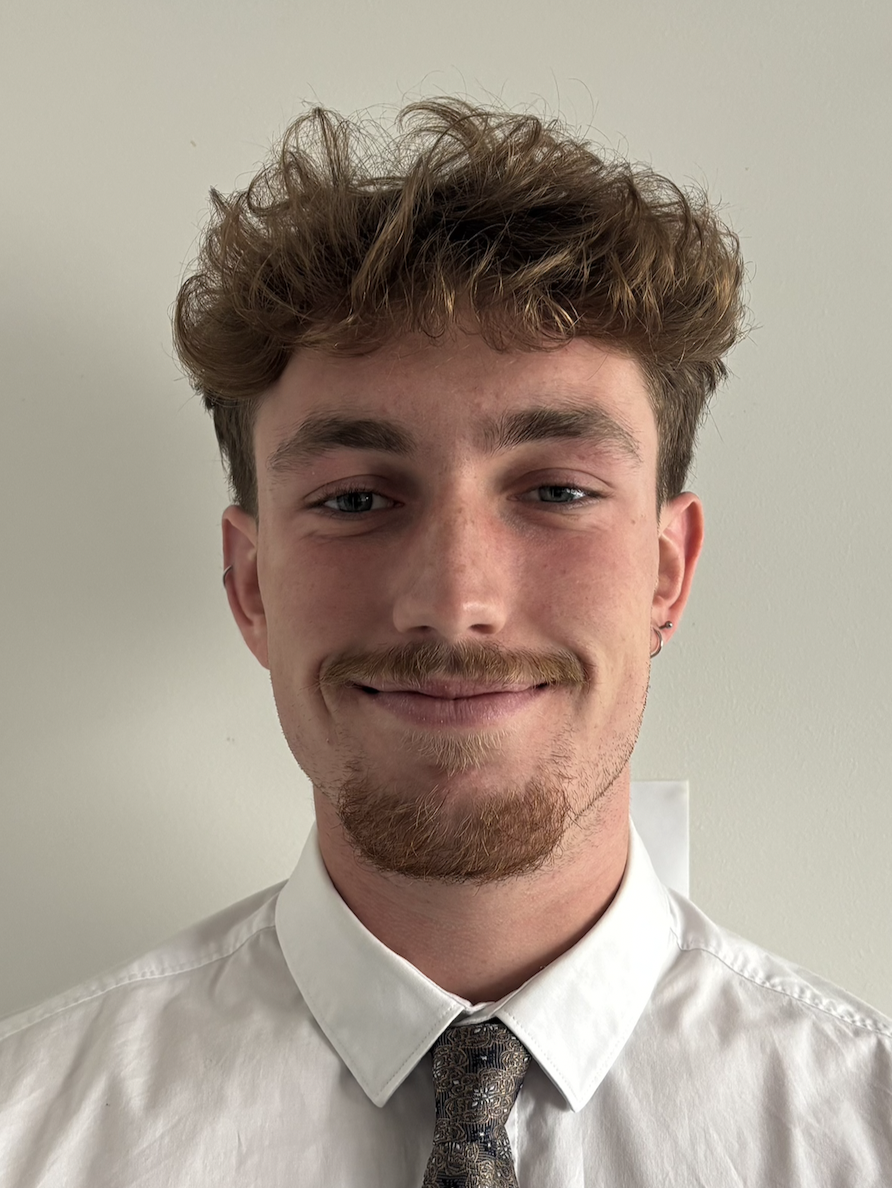
\includegraphics[width=4cm]{Photo id.png}
}
\end{tabularx}
\csection{Summary}{\small
    \begin{itemize}
        \item \footnotesize Actualmente estudiante en el INSA de Rouen
Normandía, estoy buscando realizar un
pasantía como asistente de ingeniero. Motivado, yo
estoy decidido a enriquecer mis
experiencias profesionales por el
a través de misiones de ingeniería y de
situación de "middle management"
. Yo me gustaría realizar mi pasantía de
principios de julio a mediados de septiembre. Movilidad
Francia.
    \end{itemize}
}
\csection{EDUCATION}{\small
    \begin{itemize}
        % item 1 %
        \item \textbf{Intercambio\hspace{36em}(2026)}\newline{UNCUYO - Mendoza}\newline{Carrera Industrial}{}

        \item \textbf{Diploma de ingenieria\hspace{28.5em}(2022 - 2027)}\newline{INSA Rouen Normandie}\newline{Carrera Mecanica}{}
        
        \item \textbf{Baccalauréat Général \hspace{29em}(2019-2020)}\newline{Lycée Galilée - Franqueville-Saint-Pierre}\newline{Especialidades Matematicas y Fisica-Quimica}
        
       
        
        % \item\textbf{High School\hspace{31.65em}(20xx - 20xx)}\newline{Your School.}\newline{Marks/CGPA: your marks/cgpa}{}
        
    \end{itemize}
}
 
\csection{SKILLS}{\small
    \begin{itemize}
        \item \textbf{Computacion (python, Pascal, C++, matlab)} 
        \item \textbf{Simulacion : AnSys, Catia, Solidworks} 
        % {\footnotesize AWS, Azure}{}{}
        \item \textbf{Dinamismo, espiritu de equipo y saber vivir} 
        % {\footnotesize MYSQL, MongoDB}{}{}
        \item \textbf{Ingles B2/C1 (TOEIC : 980/990)}
        % {\footnotesize Data Science and Analysis, Machine Learning, Quantum Computing}
        \item \textbf{Carnet de conducir} 
    \end{itemize}
}
    
\csection{EXPERIENCIAS}{\small
    \begin{itemize}
        \item \textbf{Intermarché \hspace{22em}Abril 2025 - Mayo 2025 (1 mes)}\newline{Vendedor}{}{}{}
        \item \textbf{Renault Cléon \hspace{18em}Julio 2023 - Augusto 2023 (1 mes)}\newline{Pasantia laboral - Operador de produccion}{}{}{}
        \item \textbf{IKEA \hspace{22em}Julio 2024 - Augusto 2024 (1 mes)}\newline{Vendedor}{}{}{}
        \item \textbf{Ibis Hotel \hspace{22em}Augusto 2023 (2 semanas)}\newline{Camarero}{}{}{}
    \end{itemize}
}
    
    % \begin{itemize}
    %     \item \textbf{Cambridge Business English Preliminary} 
    %     {\footnotesize \hspace{20em}Overall Score: 146}{}{}
    % \end{itemize}
    
    % \begin{itemize}
    %     \item \textbf{AWS Certified Developer Associate} 
    %     {\footnotesize \hspace{23.25em}Overall Score: 749}{}{}
    % \end{itemize}
    
    % \begin{itemize}
    %     \item \textbf{Certified Entry-Level Python Programmer} 
    %     {\footnotesize \hspace{20em}Overall Score: 88\%}{}{}
    % \end{itemize}
    
    % \begin{itemize}
    %     \item \textbf{Wipro TalentNext Java J2EE Certification} 
    %     {\footnotesize \hspace{20.5em}Overall Score: 78\%}{}{}
    % \end{itemize}

        




\end{document}